% Overleaf: paste this file into main.tex and select XeLaTeX.
% No external figures or bibliography file are needed.
% Prepared for Group 26. The complete report must remain within five pages.
\documentclass[11pt,a4paper]{article}
\usepackage[margin=20mm]{geometry}
\usepackage[T1]{fontenc}
\usepackage{lmodern,microtype}
\usepackage{booktabs,tabularx,array}
\usepackage{enumitem,titlesec}
\usepackage{tikz}
\usetikzlibrary{arrows.meta}
\usepackage{xurl}
\usepackage[hidelinks]{hyperref}
\hyphenation{OpsReplay}
\newcommand{\Group}{Group 26}
\newcommand{\Members}{Lee Hao Zhe, Neeraj Kumbar, Neo Qi Hao, Poh Yu Wen, See Yang Zhi, Teo Kai Xiang}
\newcolumntype{Y}{>{\raggedright\arraybackslash}X}
\setlength{\parindent}{0pt}
\setlength{\parskip}{4pt}
\setlength{\emergencystretch}{1em}
\setlist{nosep,leftmargin=*}
\titlespacing*{\section}{0pt}{9pt}{4pt}
\titlespacing*{\subsection}{0pt}{7pt}{3pt}
\renewcommand{\arraystretch}{1.12}
\hypersetup{pdftitle={OpsReplay: CS5224 Preliminary Report},
  pdfauthor={CS5224 Group 26}}

\begin{document}
\noindent
\begin{minipage}[t]{0.60\linewidth}
  \raggedright
  {\LARGE\bfseries OpsReplay}\\[3pt]
  {\small Learn production failures by investigating them.}
\end{minipage}\hfill
\begin{minipage}[t]{0.38\linewidth}
  \raggedleft\small
  \textbf{CS5224 Preliminary Report}\\[2pt]
  \Group
\end{minipage}
\par\vspace{5pt}
{\footnotesize\Members\par}
\vspace{2pt}\hrule\vspace{4pt}

\section{Motivation and Business Case}
\textbf{Theme: cloud-based production-engineering education.}

\subsection{Problem Statement and Formulation}
Students and junior engineers need opportunities to practise responding to
production failures before they become responsible for live services.
Reading an incident report explains what happened, but does not require
the reader to investigate incomplete evidence or decide how to recover a
service. In a real incident, a decision can also change the problem itself.
An attempted fix may provide temporary relief, create another failure, or
make recovery harder.

The learning problem therefore includes both diagnosis and judgement.
Learners must decide which signals matter, identify a likely cause, and
predict how an intervention will affect the system. They must then assess
the result and revise their approach. Google's Wheel of Misfortune supports
this practice through team exercises that reenact incidents from previous
postmortems~\cite{sre-postmortem}. Google's guidance also recommends reviewing
drill outcomes to identify lessons and gaps~\cite{sre-response}.

\subsection{Purpose, Target Users, and Proposed Value}
OpsReplay is a production-engineering learning platform with three modes:
\textbf{Learn}, \textbf{Challenges}, and \textbf{Code Review}. Its primary
users are computer science students, along with junior
software, DevOps, platform, and site reliability engineers. Learn explains
documented failures. Code Review develops the ability to identify risky
changes. Challenges provide practice investigating and recovering a
simulated service.

OpsReplay adapts this training approach for individual practice in a web
browser. Prepared scenarios and automated feedback let learners practise
without arranging a team exercise. The simulation models lasting action
effects and lets learners replay selected decisions to compare outcomes.

For example, scaling an application with a connection leak may overload a
shared database and disrupt another service. A later rollback stops the leak,
but queued work still delays recovery. An earlier rollback may avoid that
disruption. After an attempt, learners can return to a saved decision point,
try another action, and compare recovery time, service impact, and the causal
explanation. The intended benefit is stronger reasoning about action order
and recovery, which the evaluation in Section~\ref{sec:evaluation} will assess.

\section{Business Model}
All Learn material will remain free, including summaries and links to
official sources. A Pro subscription will unlock the team-authored Challenges
and Code Review exercises, including their feedback and debriefs. Institutional
access will license the same exercise library to a class or training cohort
at a charge per seat. The paid value is the authored practice experience.

Initial adoption will focus on students and junior engineers. Content
development, cloud hosting, and language-model use are the main costs.
Prices and willingness to pay remain unvalidated. The pilot will assess
learning value and interest in further exercises, while system measurements
will estimate the cost of delivering a session.

\newpage
\section{Architecture and Implementation}
\subsection{Learning Modes and User Experience}
Learn will provide categories, team-written summaries, lessons, and links to
official incident reports. Code Review will present a code diff with context.
Learners will identify risky lines and explain their concerns, then compare
their findings with prepared feedback. They can filter exercises by the
programming languages available in the library.

Both Challenges and Code Review will have Easy, Medium, and Hard tiers.
Difficulty will reflect evidence ambiguity, service dependencies, and the
subtlety of defects. The initial library will stay small. These modes support
studying failures, responding to them, and identifying risky changes.

Challenges are single-player exercises and the main development focus. Each
begins with an alert and limited evidence. A monitoring dashboard shows metrics,
while a resource explorer provides health, logs, events, configuration, and
deployments. Learners inspect evidence, form a hypothesis, and apply mitigation
until recovery or failure. Metrics and events share one simulated clock, with
actions marked on charts so learners can connect decisions to observed changes.

\subsection{Evolving Scenario Engine}
Each Challenge models only the factors relevant to its failure. Structured
definitions specify initial state, permitted actions, time costs, metric
rules, event conditions, and recovery or failure criteria. A deterministic
state machine uses variables and transition rules so paths can converge or
diverge. Lasting state, such as accumulated work, makes action order matter.

For each valid action, the engine applies its effect, advances simulated
time, evaluates rules, and records events. Defined time steps capture
threshold crossings and delayed effects. New investigation requests can
consume time, so an untreated incident can worsen during diagnosis. Metrics
derive from state rules and logs use authored templates. Actions and explicit
time advances drive the simulation. Rereading evidence, browser waiting, and
AI response delays do not advance time. No continuous simulation process is needed.

Table~\ref{tab:paths} shows a proposed connection-leak Challenge in which
checkout and payment share a database. Each path begins from the same state.

\begin{table}[ht]
\centering\small
\begin{tabularx}{\linewidth}{@{}>{\raggedright\arraybackslash}p{30mm}Y@{}}
\toprule
\textbf{Action sequence} & \textbf{Modelled effect} \\
\midrule
Roll back early & Replace leaking processes and close their connections before shared capacity is exhausted. \\
Scale, then roll back & Extra instances exhaust connections and disrupt payment. Rollback stops the leak, but queued work must still drain. \\
Restart application & Leaked connections close and pressure eases. The faulty version remains, so the leak returns. \\
\bottomrule
\end{tabularx}
\caption{Action order and lasting effects change the recovery path.}
\label{tab:paths}
\end{table}

The same scenario version and ordered actions, including simulated time
advances, produce the same states, metrics, events, and scores.

\subsection{Direct Controls and Conversational Interaction}
Direct controls let learners choose resources, evidence, and mitigation
parameters. An optional large language model (LLM) maps natural-language
requests to the same typed operations, such as \texttt{get\_metric} and
\texttt{scale\_service}. The backend validates parameters and prerequisites,
executes the operation, and
returns the result for the model to explain. Learners confirm proposed
mitigation before execution. Each LLM call receives current visible state,
revealed evidence, permitted tools, and relevant history, including manual
actions. Unrevealed scenario data stays outside the prompt. The engine owns
state, consequences, and scores.

\newpage
\subsection{Proposed AWS Deployment}
Figure~\ref{fig:cloud} shows the proposed deployment. Independent sessions
allow a class to practise the same Challenge without sharing incident state.
Short simulation requests suit on-demand compute, while separate LLM handlers
allow limits on slower conversational requests.

\begin{figure}[ht]
\centering
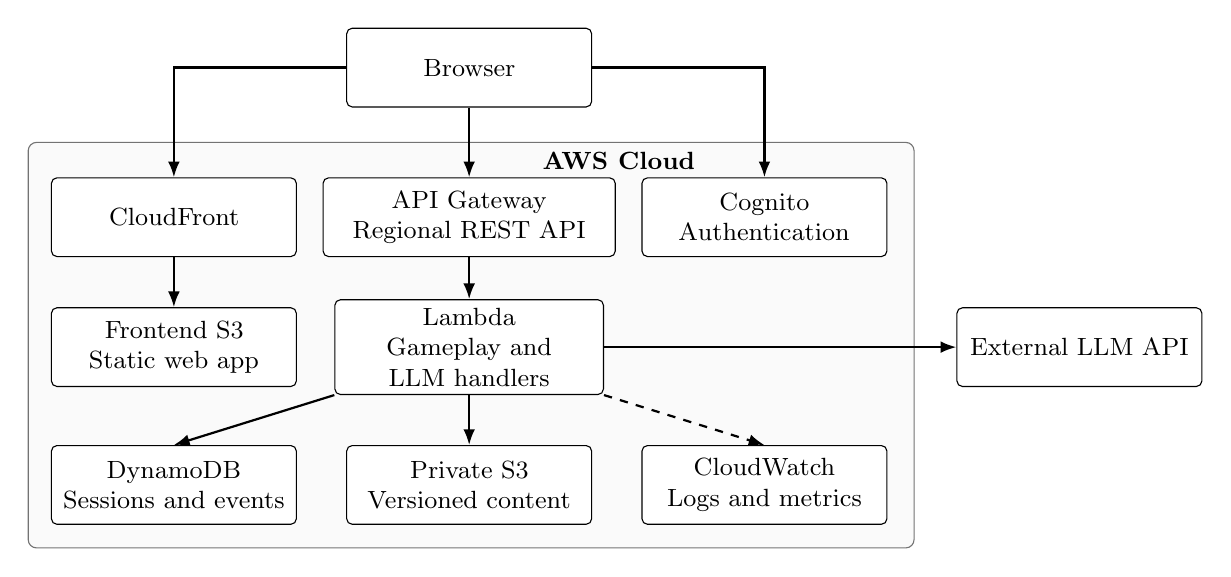
\begin{tikzpicture}[
  box/.style={draw,fill=white,rounded corners=2pt,align=center,font=\small,
    text width=29mm,minimum height=10mm,inner sep=3pt},
  flow/.style={-{Latex[length=2mm]},thick}]
\draw[rounded corners=3pt,draw=black!55,fill=black!2]
  (-6.85,-0.95) rectangle (4.4,-6.1);
\node[font=\small\bfseries] at (0.65,-1.18) {AWS Cloud};
\node[box] (browser) at (-1.25,0) {Browser};
\node[box] (cdn) at (-5,-1.9) {CloudFront};
\node[box] (web) at (-5,-3.55) {Frontend S3\\Static web app};
\node[box] (auth) at (2.5,-1.9) {Cognito\\Authentication};
\node[box,text width=35mm] (api) at (-1.25,-1.9) {API Gateway\\Regional REST API};
\node[box,text width=32mm] (lambda) at (-1.25,-3.55)
  {Lambda\\Gameplay and LLM handlers};
\node[box] (db) at (-5,-5.3) {DynamoDB\\Sessions and events};
\node[box] (private) at (-1.25,-5.3) {Private S3\\Versioned content};
\node[box] (watch) at (2.5,-5.3) {CloudWatch\\Logs and metrics};
\node[box] (llm) at (6.5,-3.55) {External LLM API};
\draw[flow] (browser.west) -| (cdn.north);
\draw[flow] (cdn) -- (web);
\draw[flow] (browser.east) -| (auth.north);
\draw[flow] (browser) -- (api);
\draw[flow] (api) -- (lambda);
\draw[flow] (lambda.south west) -- (db.north);
\draw[flow] (lambda) -- (private);
\draw[flow,dashed] (lambda.south east) -- (watch.north);
\draw[flow] (lambda.east) -- (llm.west);
\end{tikzpicture}
\caption{Requests and responses use the solid paths. The dashed arrow shows
application monitoring. The API exposes only permitted content and evidence.}
\label{fig:cloud}
\end{figure}

S3 and CloudFront will serve a static web application. Cognito will identify
users, while the backend checks session ownership and exercise access.
Private S3 will hold versioned content and hidden scenario data. CloudWatch
will monitor the application separately from the simulated incident dashboard.

A Regional API Gateway REST API will route requests to stateless Lambda
handlers. The message route will stream responses while preserving the full
tool-selection, execution, and explanation loop. AWS supports response
streaming for REST APIs, while the cheaper HTTP API lacks streaming and has a
30-second integration limit~\cite{aws-api}. An early deployment test will
verify runtime and regional support. Streaming improves feedback but does
not reduce model computation. Lambda remains billed while waiting, even
after a client disconnects~\cite{aws-streaming}. Provider timeouts, token
limits, and separate concurrency budgets will bound AI use and preserve
capacity for direct actions.

DynamoDB fits session-based access without relational joins. It will store
progress, review submissions, and conversation history. Each session will
have a bounded state record, separate ordered events, and stored request
results. A transaction will update state, append an event record, and save
the result under a request ID. Retries will retrieve that result without
repeating effects. Version checks will reject stale actions, including tools
selected before a direct action changed the session. Completed actions remain
retrievable if an LLM explanation fails. Replay will create a separate session
from a saved checkpoint, preserving the original attempt and scenario version.

This design reduces idle compute and server maintenance, but introduces cold
starts, service quotas, and AWS-specific integration. A single-server
application with PostgreSQL has fewer deployment components and more flexible
queries, but requires provisioned capacity and server maintenance. It may
suit sustained traffic better. The proposed serverless design targets
intermittent training demand.
The engine will remain separate from cloud access code. Local storage adapters
will support testing before deployment. An AWS test deployment will then
verify authentication, permissions, persistence, and streaming. This separation
also supports an equivalent on-premise implementation.

\newpage
\subsection{Implementation Plan}
The team will first prove one complete Challenge, then add a small Learn
collection and Code Review set. Expansion will follow content validation.

\begin{table}[ht]
\centering\small
\begin{tabularx}{\linewidth}{@{}p{30mm}Y@{}}
\toprule
\textbf{Period (2026)} & \textbf{Planned deliverable} \\
\midrule
21--28 Sep & Finalise the reference scenario and submit the preliminary report. \\
29 Sep--11 Oct & Build the engine and test lasting effects, checkpoints, and deterministic replay. Validate AWS transport. \\
12--25 Oct & Integrate the interface, persistence, replay comparison, debrief, and LLM. Add Learn content and tiered Code Review with language filters. \\
26 Oct--5 Nov & Validate additional content and run system tests and the learner study. \\
6--13 Nov & Resolve findings and complete cost analysis, the final report, slides, and demonstration. \\
\bottomrule
\end{tabularx}
\caption{Proposed delivery schedule, with Challenges receiving most development effort.}
\end{table}

\subsection{AI Teaching Support}
The LLM will offer concept explanations using visible evidence and hints
released by the backend. After submission, it can explain reference findings
and the debrief. It will not set scores or grade free-text reasoning. AI and
hint use will be recorded to distinguish assisted results. Direct controls
and prepared feedback remain available if the provider fails.

\subsection{Scoring, Debrief, and Replay}
Exercises will use original artefacts inspired by documented failures and
link to official sources. Challenge scoring will consider investigation effort,
recovery time, and cumulative service impact. Reduced impact counts even when
the root cause remains. The debrief will explain key and missed evidence,
action effects, the root cause, and recommended recovery using recorded events.

After an attempt, learners can replay from a few authored checkpoints and
compare paths from the same state. The comparison will show recovery time,
service impact, and why outcomes differ. The original history and score will
remain unchanged. Replay is informed practice after the debrief, so its results
will be labelled separately from the first attempt.

\section{Evaluation Plan}
\label{sec:evaluation}
Results will identify scenario versions, deployment settings, and sample size.

\subsection{System Correctness, Reliability, and Performance}
\begin{itemize}
\item \textbf{Correctness.} Repeat fixed actions and compare states, metrics,
events, and scores. Test action order, delayed effects, temporary relief, and
checkpoint restoration. Verify that replay preserves the first attempt,
interface values match state, and content references and answers are valid.
\item \textbf{Access and reliability.} Test ownership, paid access, hidden
evidence, stale actions, duplicate requests, interrupted writes, and provider
failures. Retries must not repeat effects or score penalties.
\item \textbf{Performance.} Measure median and 95th-percentile latency,
throughput, errors, and database throttling at 10, 50, and 100 independent
sessions. Record action mix and think time. These are proposed test loads.
\end{itemize}

\subsection{LLM Accuracy, Latency, and Cost}
A labelled request set will specify context and acceptable tools and arguments.
Tests will measure selection accuracy, invalid calls, unsupported claims,
answer leakage, and teaching accuracy. For each model, we will record median
and 95th-percentile latency for the full conversational loop and token cost
per session. Engine load tests will exclude provider delay, with separate
real-provider tests under a fixed budget. Simulated responses will be labelled.

\newpage
\subsection{User Evaluation}
We propose a formative pilot with 5--10 computer science students or junior
engineers. Each will investigate an incident, read its debrief, and replay a
selected decision. For another incident of similar difficulty, the learner
will read a static explanation that includes alternative actions and outcomes.
We will balance assignment and order as far as the sample permits, allow equal
study time, and provide equivalent causal information. Direct controls without
AI will isolate the simulation and replay workflow from teaching assistance.

Questions before and after each condition will assess diagnosis and causal
reasoning using a common rubric. Before replay, learners will predict how a
different action changes recovery. Afterward, they will explain the result and
apply the lesson to a new decision. We will record completion, harmful actions,
and explanation quality. Brief tasks will check Learn, Code Review, and optional
AI support. Participants will complete the System Usability Scale
(SUS)~\cite{sus} and a short interview on usability and replay usefulness.

Results will report individual scores, paired differences, and usability
problems. The pilot can guide improvement and provide early learning evidence.
It cannot establish broad effectiveness, long-term retention, or the separate
effect of replay within the full workflow.

\subsection{Cloud Cost and On-Premise Comparison}
The preliminary choice of serverless hosting assumes intermittent demand.
We will compare steady use and class-sized bursts with an on-premise deployment
of the same service. The final report will use measured workloads and published
rates. AWS costs will include API requests, compute, database, storage, transfer,
authentication, and monitoring. On-premise costs will
include suitable hardware spread over its useful life, power, networking,
maintenance, and staff time. Both will use the same external LLM and include
its cost. We will report cost per completed session, capacity, and availability
assumptions. Credits will be separate, without assuming cloud hosting is cheaper.

\section{Conclusion}
OpsReplay combines free learning with authored practice. Its main focus is an
evolving incident with lasting consequences and replay of recovery decisions.
The team will prove one complete Challenge before expanding the library and
evaluating usability, learning, reliability, and cost. The plan assumes access
to testers and an LLM provider with function calling. Exercise counts, available
languages, scoring weights, model choice, and prices remain open.

\begingroup
\small
\begin{thebibliography}{9}
\setlength{\itemsep}{2pt}
\bibitem{sre-postmortem}
Google, ``Postmortem Culture: Learning from Failure,''
\textit{The Site Reliability Workbook}.\newline
\url{https://sre.google/workbook/postmortem-culture/}.
\bibitem{sre-response}
Google, ``Incident Response,'' \textit{The Site Reliability Workbook}.\newline
\url{https://sre.google/workbook/incident-response/}.
\bibitem{aws-api}
AWS, \href{https://docs.aws.amazon.com/apigateway/latest/developerguide/http-api-vs-rest.html}{``Choose Between REST APIs and HTTP APIs''} and
\href{https://docs.aws.amazon.com/apigateway/latest/developerguide/http-api-quotas.html}{``Quotas for HTTP APIs,''}
\textit{API Gateway Developer Guide}.
\bibitem{aws-streaming}
AWS, \href{https://docs.aws.amazon.com/apigateway/latest/developerguide/response-transfer-mode.html}{``Stream the Integration Response''} and
\href{https://docs.aws.amazon.com/lambda/latest/dg/configuration-response-streaming.html}{``Response Streaming for Lambda Functions,''}
\textit{AWS Documentation}.
\bibitem{sus}
J. Brooke, ``SUS: A `quick and dirty' usability scale,''
in \textit{Usability Evaluation in Industry}, 1996, pp.~189--194.
\end{thebibliography}
Web references accessed 21 September 2026.

\medskip
\textbf{AI-use declaration.}
The team developed the project concept and selected the design direction. AI
assisted with design evaluation, reference checks, report drafting, language
refinement, and LaTeX preparation. This work clarified the distinction between
repeatable simulation results and learning outcomes that require user evaluation.
\endgroup
\end{document}
